\documentclass{beamer}
\label{key}\usetheme{Boadilla}
\usepackage{ dsfont }
%\usepackage{ tipa }

\title{Nonlinear Observer for Tightly Coupled Integration of Pseudorange and Inertial Measurements}
\subtitle{Guide and Navigation Systems}
\author{Pietro Bramante, Liana Bertoni, Fulvio Di Luzio}
\institute{Universit\`a degli Studi di Pisa \\ Master's Degree in Robotics and Automation Engineering}
\date{\today}






\begin{document}
	
	\begin{frame}
	\titlepage
	\end{frame}	


	\begin{frame}
		\frametitle{Outline}
		\tableofcontents
		
		\section{Introduction}
		\section{Models}
			\subsection{Vehicle Kinematics}
			\subsection{Inertial Sensor Models}
			\subsection{Pseudorange Measurement Model}
		\section{Observer Design}
			\subsection{Attitude Observer}
			\subsection{Translation Motion Observer}
			\subsection{Stability and Selection of Gain Matrix}
		\section{Implementation Design}
		\section{Case Study}	
	\end{frame}

	\begin{frame}
		\frametitle{Introduction}
		This presentation shows the obtained results by the implementation of the article written by Tor. A. Johansen and Thor I. Fossen.
		\vspace{0.5cm}
		
	\begin{figure}[H]
			\centering
			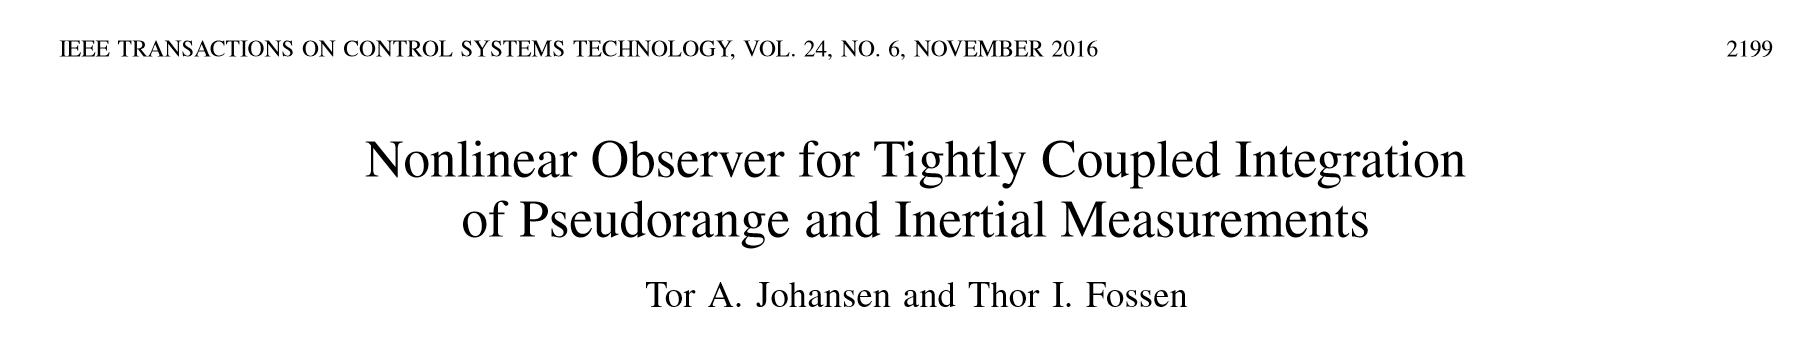
\includegraphics[scale=0.3]{title}
			%\caption{Block diagram of the closed-loop system for $\mu$ analysis and synthesis. \label{fig::title}}
		\end{figure}
	\end{frame}

	\begin{frame}
		\frametitle{Introduction}
	%	The work has been developed in Matlab and Simulink (v. R2016b).
	The goal of navigation systems is to estimate the vehicle position within a certain area. This is let generally by a inertial navigation system, based on $IMU$ (Inertial Measurement Unit).\\
	
	Using an interconnection of a nonlinear attitude observer and a translational motion observer based on pseudorange and range-range measurements, a tightly coupled integrated aided inertial navigation system is designed!?!?!?\\
	
	Due to the problem of measurements integration, this method is supported by other techniques. In this work, the inertial navigation system is aid by pseudorange measurements, obtained by transponders.
	%The article shows hot to build an inertial navigation  system  with the aid of pseudorange measurements, obtained by proper transponders.
	\end{frame}


	\begin{frame}
	\frametitle{Vehicle Kinematics}
	The vehicle kinematic model is given by
	
	\[ \dot{p^n} = v^n \]
	
	\[ \dot{v^n} = R^n_b f^b + g^n\]
	
	\[ \dot{R^n_b} = R^n_bS(\omega^b_{ib}) \]
	
	Where $p^n$, $v^n$, $f^n$ are position, velocity and proper acceleration in NED (North-East-Down), respectively, while the attitude is described by a rotation matrix $R^n_b$ that represents the rotation from \textit{body} to NED; $\omega^b_{ib}$ represents the rotation rate of body with respect to ECI (Earth-Centered-Inertial) and $g^n$ denotes the gravity vector. We also assume NED to be an inertial frame. 
	
	\end{frame}
	
	\begin{frame}
	\frametitle{Inertial Sensor Models}
	The inertial sensor model is based on the strapdown assumption
	
	\[ f^b_{IMU} = f^b + \epsilon_f\]
	
	\[ \omega^b_{ib,IMU} = \omega^b_{ib} + b + \epsilon_\omega \]
	
	\[ \dot{b} = \epsilon_b \]
	
	\[ m^b_{mag} = m^b + \epsilon_m \]
	
	where $\epsilon_f$, $\epsilon_\omega$ and $\epsilon_m$ account for noise, and $b$ denotes the rate gyro bias that is driven by the noise $\epsilon_b$ and assumed to be bounded.  
	\\ All sensors are 3-D.
	\end{frame}
	
	\begin{frame}
	\frametitle{Pseudorange Measurement Model}
	
	The geometric range 
	
	\[ \rho_i = \|p^n - p^n_i\|_2 \]
	
	is a nonlinear function of the vehicle position $p^n$ and the $i$th transponder position $p^n_i$, given by their Euclidean distance.
	\\ The pseudorange measurement model is
	
	\[ y_i = \rho_i + \beta + \epsilon_{yi} \]
	
	where $\beta \in \mathds{R}$ is a bias parameter due to unknown clock synchronization errors or other unknown effects and $\epsilon_{yi}$ the noise.
	\\ $i = 1,2,...,m$ where $m$ is the number of measurements.
	\end{frame}
	
	\begin{frame}
	\frametitle{Pseudorange Measurement Model}
	The nonlinear model can be approximated with a linear one by an algebraic transformation 
	
		\[ 2C_{\delta x}x = \delta + \varepsilon  \]
		
	where the matrix $C_{\delta x} \in \mathds{R}^{(m-1)\times4}$ is
	
	$$
	C_{\delta x} :=
	\begin{pmatrix}
	(p^n_m - p^n_1)^T & y_1 - y_m \\
	\vdots \\
	(p^n_m - p^n_{m-1})^T & y_{m-1} - y_m 
	\end{pmatrix} 
	$$
	
	$\varepsilon \in \mathds{R}^{m-1}$ the noise and $\delta \in \mathds{R}^{m-1}$ the vector of squared range measurements. \\ $x := (p^n_\Delta;\beta)$ where $p_\Delta^n = p^n - p^n_0$ ($p_\Delta^n$ is a reference point in NED). 
	\end{frame}

	\begin{frame}
	\frametitle{Observer Design}
	Two observer are designed: one for the attitude estimation and one for the translational motion estimation. 
		\begin{figure}[H]
		\centering
		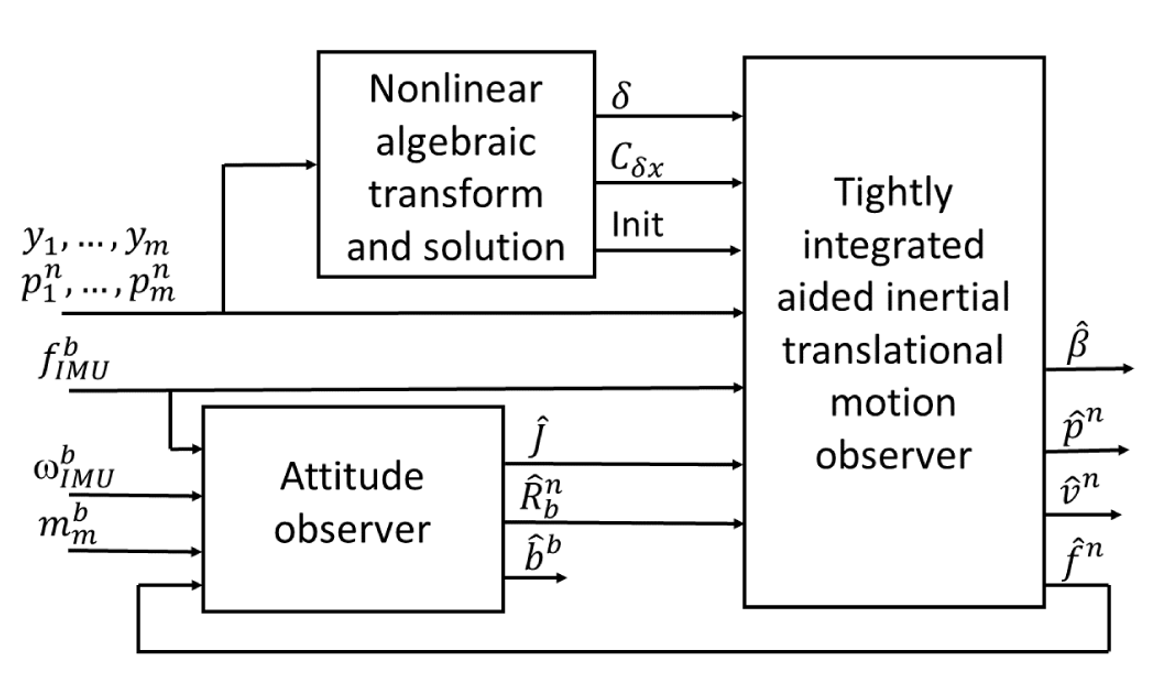
\includegraphics[scale=0.3]{observers}
		\caption{Overall block diagram for tightly integrated observer.}
	\end{figure}
	\end{frame}

	\begin{frame}
		\frametitle{Attitude Observer}
		The attitude variables to estimate are $R^n_b$ and $b$.
		
		\[ \dot{\hat{R}}^n_b  =  \hat{R}^n_b S(\omega^b_{ib,IMU} - \hat{b}) + \sigma K_pJ(t, \hat{R}^n_b)       \]
		
		\[ \dot{\hat{b}} = Proj(-k_I vex(\mathds{P}_a (sat(\hat{R}^n_b)^T K_P J(t, \hat{R}^n_b))),M_{\hat{b}} )           \]
		
		where $K_P > 0 \in \mathds{R}^{3\times 3}$ is a symmetric gain matrix, $K_I > 0$ is a scalar gain and $\sigma \geq 1$.\\ 
		
		The function $sat(\cdot)$ is an element-wise saturation, while $Proj(\cdot)$ is a parameter projection which ensures that $\|\hat{b} \|_2$ is bounded.
	\end{frame}

	\begin{frame}
 		\frametitle{Attitude Observer}
 		The function $J(\cdot) \in  \mathds{R}^{3\times 3}$ is a stabilizing injection term
 		
 		\[ J(t, \hat{R}^n_b)  = (E^n - \hat{R}^n_b E^b)(E^b)^T    \]
 		
 		based on the vector measurements $m^b_{mag}$ and $f^b_{IMU}$  and their NED reference vetors $m^n$ and $\hat{f}^n$ used to define vectors scaled by nonzero terms
 		
 		\[ q_1^b = m^b_{mag}/\|m^b_{mag}\|_2 \qquad q_2^b = f^b_{IMU}/\|g^n\|_2    \]
 		
 		\[ q_1^n = m^n/\|m^n\|_2 \qquad q_2^n = \hat{f}^n/\|g^n\|_2    \]
 		
 		and the $3\times3$ matrices
 		
 		\[ E^b = (q_1^b, S(q^b_1)q_2^b, S^2(q_1^b)q_2^b)    \]
 		
 		\[ E^n = (q_1^n, S(q^n_1)q_2^n, S^2(q_1^n)q_2^n)    \]
	\end{frame}


	\begin{frame}
		\frametitle{Translational Motion Observer}
		The variables to estimate are $p^n$,$v^n$,$f^n$,$\beta$.
		
		\[ \dot{\hat{p}}^n_\Delta = \hat{v}^n + K_{pp}(\delta - \hat{\delta})  \]
		
		\[ \dot{\hat{\beta}} = K_{\beta p} (\delta - \hat{\delta}) \]
		
		\[ \dot{\hat{v}}^n = \hat{f}^n + g^n + K_{vp}(\delta - \hat{\delta})\]
		
		\[ \dot{\xi} = - \sigma K_P J(t, \hat{R}^n_b)f^b_{IMU} + K_{\xi p}(\delta - \hat{\delta}) \]
		
		\[ \hat{f}^n = \hat{R}^n_b f^b_{IMU} + \xi  \]
		
		where $\hat{\delta} = 2C_{\delta x}\hat{x}$ and the gain matrix $K \in \mathds{R}^{10\times(m-1)}$ is made of the matrices $K_*$ and is in general time varying.
	\end{frame}

	\begin{frame}
		\frametitle{Translational Motion Observer}
		Then it is possible to build the \textit{estimated state} vector $\dot{\tilde{\chi}} = (\tilde{p}^n_\Delta;\tilde{\beta}; \tilde{\hat{v}}^n; \tilde{\hat{f}}^n) \in \mathds{R}^{10}$ and the relative LTV error system
		
		\[ \dot{\tilde{\chi}} = (A - KC)\tilde{\chi} + Bu + B\epsilon_u + K\varepsilon\]
		
		\[ u = \tilde{R}^n_b \dot{f}^b + \tilde{R}^n_b S(\omega^b_{ib})f^b - \hat{R}^n_b S(\tilde{b})f^b\]
	\end{frame}

	\begin{frame}
		\frametitle{Translational Motion Observer}
		The matrices $A \in \mathbb{R}^{10\times 10}$,$B \in \mathbb{R}^{10\times 3}$,$C \in \mathds{R}^{(m-1) \times 10} $ and $K \in \mathds{R}^{10 \times (m-1)}$ are described as follows
		$$
		A :=
		\begin{pmatrix}
		0 & 0 & I_3 & 0 \\ 
		0 & 0 & 0 & 0 \\
		0 & 0 & 0 & I_3 \\
		0 & 0 & 0 & 0
		\end{pmatrix}
		\qquad
		B := 
		\begin{pmatrix}
		0 \\ 0 \\ 0 \\ I_3
		\end{pmatrix}
		$$
		
		$$
		K := 
		\begin{pmatrix}
		K_{pp} \\ K_{\beta p} \\ K_{vp} \\ K_{\xi p}
		\end{pmatrix}
		\qquad
		C :=
		\begin{pmatrix}
		2C_{\delta x} & 0 & 0
		\end{pmatrix}
		$$
	\end{frame}

	\begin{frame}
		\frametitle{Translational Motion Observer}
		The gain matrix $K$ is time varying and calculated as
		
		\[ K := PC^TR^{-1} \]
		
		 where $P$ is solution of the $Riccati$ equation
		
		\[ \dot{P} = PA + A^TP - PC^TR^{-1}CP + Q\]
	\end{frame}
	
	\begin{frame}
		\frametitle{Implementation Design}
		The Simulink implementation is similar to the one offered by the article:
		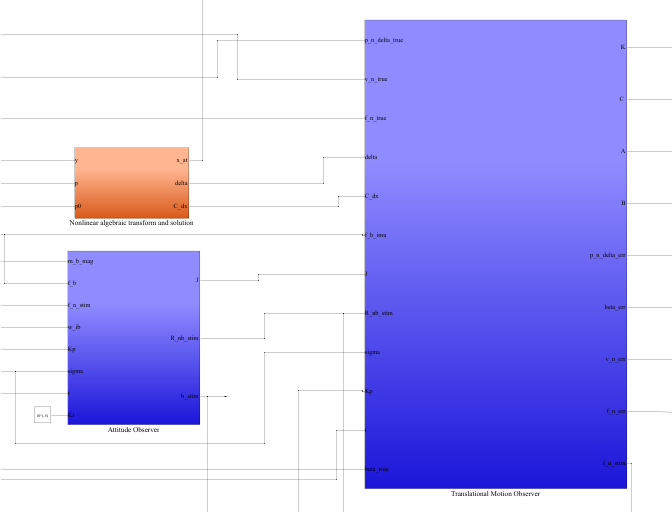
\includegraphics[scale = 0.4]{scheme}
	\end{frame}
	\begin{frame}
		\frametitle{Implementation Design}
		The Attitude Observer is made of three main function blocks:
		The first one implements the function $J(\cdot) $ as previously described. 
		The function $b\_computation$ computes the dinamics of the bias by means of the $Proj(\cdot)$ function. and the function $Rot\_func$ computes an estimate of the rotation matrix. 
		The following picture shows the Simulink scheme:
		
	\end{frame}
	
	\begin{frame}
		\frametitle{Implementation Design}
		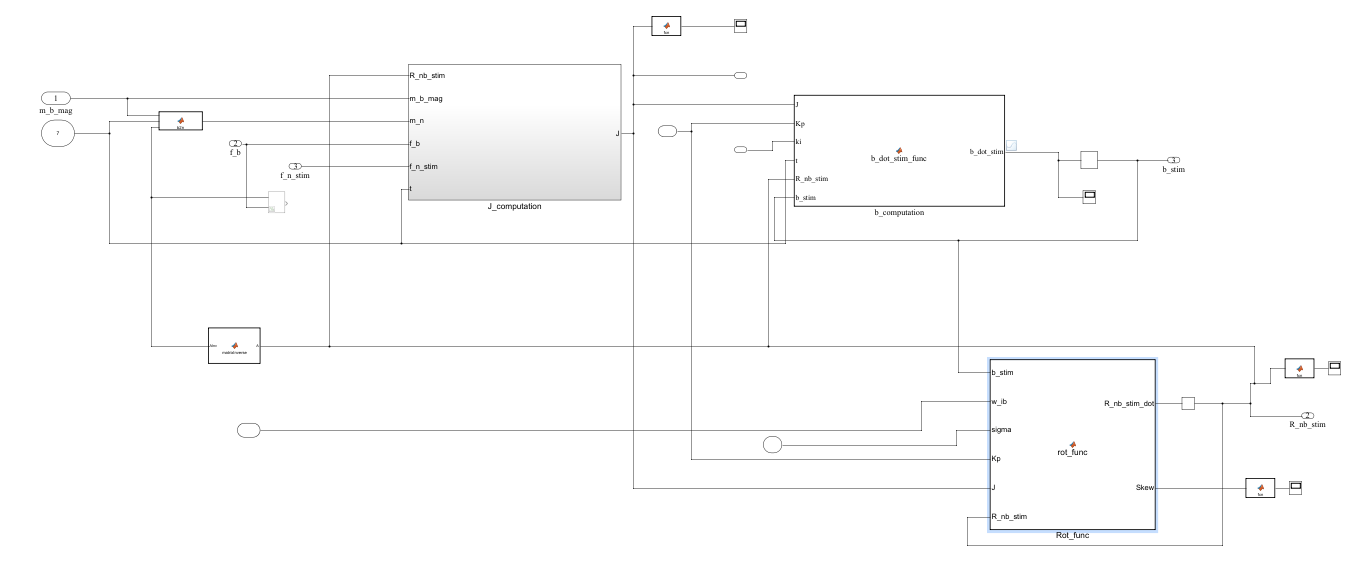
\includegraphics[scale=0.25]{at}
	\end{frame}

	\begin{frame}
		\frametitle{Implementation Design}
		The $Nonlinear Algebraic Transform$ block computes the $C_{\delta x}$ matrix and the following variable:
		
		\[\hat{x} = \frac {C_{\delta x}^{+} \delta}{2}  \]
		
		that is the unique solution to
		
		\[ 2C_{\delta x} x = \delta + \epsilon \]
		
		in the case of $m \geqslant 5$ transponders.
	\end{frame}
	
	\begin{frame}
		\frametitle{Implementation Design}
		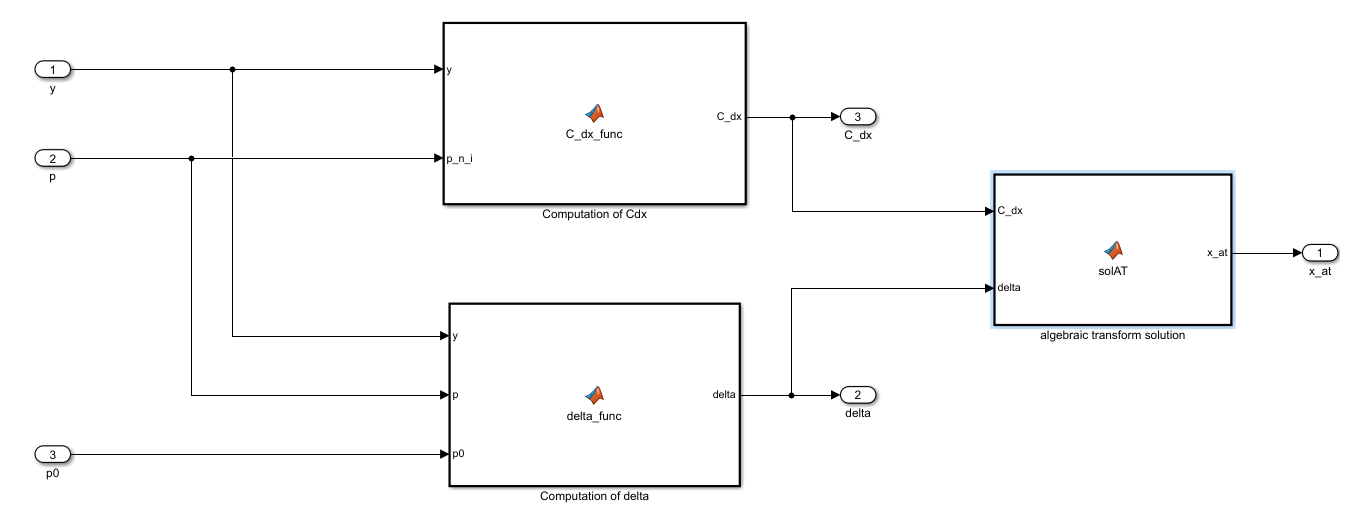
\includegraphics[scale = 0.25]{NLAT}
	\end{frame}

\end{document}